\chapter[Analýza centralít \small{(Tuan Dávid Nguyen Van)}]{Analýza centralít}
\label{centrality}

Kapitola sa venuje analýze sieťových centralít v globálnej leteckej sieti, konkrétne degree, betweenness, closeness, eigenvector a Katz 
centralite a ich využitiu na identifikáciu kľúčových uzlov


\section{Metodológia a technické spracovanie}

Pre výpočet centralít sme využili knižnicu NetworkX, ktorá poskytuje efektívne implementácie pre rôzne typy centralít
a knižnice Pandas pre štatistické spracovanie dát.

\subsection{Normalizácia}
Pre každý typ centrality sme vypočítali hodnoty pre všetky letiská v sieti a následne sme tieto hodnoty normalizovali, 
aby sme mohli porovnávať letiská medzi sebou. Normalizácia bola vykonaná pomocou min-max škálovania, ktoré transformuje
hodnoty centralít do rozsahu [0, 1] podľa vzorca:

\begin{equation}
    \text{Centrality}_{\text{norm}}(v) = \frac{\text{Centrality}(v) - \min(\text{Centrality})}{\max(\text{Centrality}) - \min(\text{Centrality})}
\end{equation}

Po normalizácii sme vytvorili nový DataFrame, ktorý obsahuje názvy letísk, ich centrality a ďalšie relevantné 
informácie, ako je kontinent, na ktorom sa nachádzajú.


\section{Definícia sieťových centralít}

Na kvantifikáciu dôležitosti uzlov sme aplikovali päť základných metrík, pričom každá zachytáva odlišný aspekt sieťovej dominancie:

\begin{itemize}

    \item \textbf{Degree Centrality ($C_D$)} -- vyjadruje počet priamych spojení daného uzla. 
    Letisko s vysokou degree centralitou disponuje veľkým počtom priamych letov na iné letiská.
    
    \item \textbf{Betweenness Centrality ($C_B$)} -- vyjadruje, cez koľko najkratších ciest medzi dvojicami uzlov prechádza daný uzol. 
    Letisko s vysokou betweenness centralitou predstavuje významný tranzitný bod siete.
    
    \item \textbf{Closeness Centrality ($C_C$)} -- charakterizuje priemernú vzdialenosť uzla od všetkých ostatných uzlov v sieti. 
    Letisko s vysokou closeness centralitou je schopné efektívne komunikovať s ostatnými letiskami.
    
    \item \textbf{Eigenvector Centrality ($C_E$)} -- hodnotí význam uzla na základe významu jeho susedných uzlov. 
    Letisko s vysokou eigenvector centralitou je prepojené s inými významnými letiskami.
    
    \item \textbf{Katz Centrality ($C_K$)} -- rozširuje eigenvector centralitu o faktor útlmu, ktorý znižuje vplyv vzdialenejších uzlov. 
    Letisko s vysokou Katz centralitou má výrazný vplyv na sieť aj nepriamo prostredníctvom vzdialenejších spojení.

\end{itemize}

\section{Kompozitné indexy (Vlastná analytická nadstavba)}
\label{sec:indexy}

V tejto sekcii definujeme vlastnú analytickú nadstavbu vo forme piatich kompozitných indexov. Keďže základné centrality sú v komplexných 
sieťach často silne korelované, zavádzame päť kompozitných indexov, ktoré ich štatisticky odfiltrujú a odhalia špecifické strategické roly 
jednotlivých letísk.

\subsection{Global Hub Score (Celková systémová dominancia)}
Tento index predstavuje normalizovaný aritmetický priemer všetkých piatich vypočítaných centralít. Slúži na identifikáciu „absolútnych“ lídrov 
siete – uzlov, ktoré dominujú vo všetkých aspektoch konektivity, tranzitu aj prestíže.
\[
\text{Global Hub Score} = \frac{1}{5} (C_D + C_B + C_C + C_E + C_K)
\]
Uzly s vysokým skóre v tomto indexe tvoria chrbticu globálnej leteckej dopravy a sú kritické pre celkovú súdržnosť a odolnosť grafu.

\subsection{Bridge Index (Strategické premostenie)}
Index identifikuje uzly, ktoré vykazujú disproporčne vysokú mieru kontroly tranzitu vzhľadom na ich relatívne nízky počet priamych spojení. 
Tieto uzly reprezentujú geografické alebo topologické „skratky“.
\[
\text{Bridge Index} = \frac{C_B}{C_D + \epsilon}
\]
Kde konštanta $\epsilon = 0,001$ zabezpečuje numerickú stabilitu pri delení. Vysoká hodnota indexu indikuje tzv. \textit{bottlenecks} 
siete, ktoré sú kritické pre integritu najkratších ciest medzi kontinentmi.

\subsection{Regional Index (Regionálna akumulácia)}
Tento ukazovateľ izoluje uzly s vysokou lokálnou konektivitou, ktoré však nedisponujú globálnym tranzitným významom. Vysoká hodnota znamená, 
že letisko slúži primárne ako regionálny zberný bod alebo cieľová destinácia.
\[
\text{Regional Index} = C_D - C_B
\]
Letiská s vysokým regionálnym indexom zvyšujú kapacitu a hustotu dopravy v rámci kontinentov, ale ich systémový vplyv na integritu globálnych 
trás je nižší.

\subsection{Prestige Index (Index sieťovej prestíže)}
Index je navrhnutý na identifikáciu tzv. „elitných satelitov“. Ide o letiská, ktoré majú nízky celkový počet spojení, ale tieto spojenia smerujú 
výhradne do najvýznamnejších svetových hubov.
\[
\text{Prestige Index} = \frac{C_E}{C_D + \epsilon}
\]
Vysoká hodnota Prestige Indexu naznačuje, že letisko je priamou bránou z periférie do jadra globálneho systému, čím získava vysokú topologickú 
prestíž napriek svojej relatívne malej veľkosti.

\subsection{Local Giant Index (Index vnútroštátnej dominancie)}
Tento index meria rozdiel medzi priamou konektivitou (Degree) a globálnou prestížou (Eigenvector). Slúži na identifikáciu masívnych uzlov, 
ktoré sú však napojené na veľký počet nízko významných (často vnútroštátnych) letísk.
\[
\text{Local Giant Index} = C_D - C_E
\]
Typickými predstaviteľmi sú veľké uzly vo vnútroštátnych sieťach (napr. USA alebo Čína), ktoré obsluhujú obrovské objemy dopravy, no v globálnom 
„elitnom klube“ najprepojenejších medzinárodných hubov hrajú sekundárnu rolu.


\section{Analýza primárnych centralít}

Pred aplikáciou kompozitných indexov sme identifikovali desať najvýznamnejších uzlov pre každú z piatich základných metrík. 
Tieto výsledky tvoria empirický základ pre našu funkčnú typológiu a odhaľujú dôležité rozdiely v charaktere jednotlivých letísk.

\subsection{Porovnanie Top 10 uzlov podľa sieťových metrík}

V tabuľke \ref{tab:top10_raw} uvádzame rebríčky letísk zoradené podľa jednotlivých centralít. Hodnoty predstavujú normalizované 
skóre v rámci celého grafu.

\begin{table}[h!]
\centering
\small
\resizebox{\textwidth}{!}{
\begin{tabular}{c|l|l|l|l|l}
\hline
\textbf{\#} & \textbf{Degree ($C_D$)} & \textbf{Betweenness ($C_B$)} & \textbf{Eigenvector ($C_E$)} & \textbf{Closeness ($C_C$)} & \textbf{Katz ($C_K$)} \\ \hline
1.  & Frankfurt & Paris       & Amsterdam & Frankfurt & Frankfurt \\
2.  & Paris     & Los Angeles & Frankfurt & Paris     & Amsterdam \\
3.  & Amsterdam & Dubai       & Paris     & London    & Paris     \\
4.  & Istanbul  & Anchorage   & Munich    & Dubai     & Istanbul  \\
5.  & Atlanta   & Frankfurt   & London    & Amsterdam & Munich    \\
6.  & Chicago   & Beijing     & Rome      & Los Angeles& Atlanta   \\
7.  & Beijing   & Chicago     & Barcelona & New York  & Beijing   \\
8.  & Munich    & Toronto     & Istanbul  & Toronto   & Chicago   \\
9.  & Moscow    & Amsterdam   & Zürich    & Istanbul  & London    \\
10. & Dallas    & Istanbul    & Madrid    & Munich    & Dubai     \\ \hline
\end{tabular}
}
\caption{\centering Porovnanie Top 10 globálnych letísk podľa piatich primárnych centralít.}
\label{tab:top10_raw}
\end{table}


Výsledky ukazujú, že jednotlivé centrality zachytávajú odlišné aspekty významu uzlov v globálnej leteckej sieti. Hoci medzi metrikami 
existuje určitá miera prekryvu, poradie letísk sa v jednotlivých rebríčkoch výrazne líši, čo naznačuje existenciu viacerých funkčných typov hubov.

Najvýraznejšie postavenie v sieti dosahujú európske uzly, predovšetkým \textbf{Frankfurt}, \textbf{Paris Charles de Gaulle} 
a \textbf{Amsterdam Schiphol}. Tieto letiská sa opakovane objavujú medzi najvyššie hodnotenými uzlami naprieč všetkými centralitami, 
čo potvrdzuje ich úlohu nielen ako veľkých dopravných centier ($C_D$), ale aj ako systémovo integrovaných uzlov s vysokou globálnou dostupnosťou 
($C_C$) a prestížou ($C_E$).

Významnú anomáliu predstavuje letisko \textbf{Anchorage}, ktoré sa umiestnilo na štvrtom mieste v rámci \textit{Betweenness centrality}, 
napriek tomu, že sa nevyskytuje v ostatných rebríčkoch Top 10. Tento výsledok naznačuje, že jeho význam nevyplýva z veľkého množstva spojení, 
ale z jeho strategickej polohy na tranzitných trasách medzi Áziou a Severnou Amerikou. Letisko tak predstavuje typ uzla, ktorého dominantná 
úloha spočíva v kontrole kritických najkratších ciest v sieti.

Odlišný charakter vykazujú aj letiská ako \textbf{Atlanta} alebo \textbf{Dallas/Fort Worth}, ktoré dosahujú vysoké hodnoty 
\textit{Degree centrality}, avšak absentujú medzi lídrami v rámci \textit{Eigenvector centrality}. To naznačuje, že ich konektivita je 
orientovaná najmä na rozsiahle regionálne alebo vnútroštátne siete, pričom ich prepojenie na globálne dominantné huby je relatívne slabšie.

Rebríček \textit{Katz centrality} vykazuje vysokú mieru podobnosti s \textit{Degree centrality}, avšak mierne zvýhodňuje uzly prepojené 
s významnými susedmi. Najvyššiu hodnotu dosahuje \textbf{Frankfurt}, čo potvrdzuje jeho stabilný systémový význam 
aj v modeli zohľadňujúcom vzdialenejšie sieťové vplyvy.

\subsection{Vizualizácia vzťahu Degree a Betweenness centrality}

Hoci rebríčky v Tabuľke \ref{tab:top10_raw} identifikujú najvýznamnejšie uzly podľa jednotlivých metrík, neposkytujú úplný pohľad na 
vzájomné vzťahy medzi konektivitou a tranzitným významom uzlov. Pre hlbšie pochopenie štrukturálnych rolí letísk sme preto zostavili 
korelačný graf (Obr. \ref{fig:degree_vs_betweenness}), ktorý zobrazuje vzťah medzi priamou konektivitou uzla ($C_D$) a jeho tranzitným vplyvom ($C_B$).

\begin{figure}[h!]
    \centering
    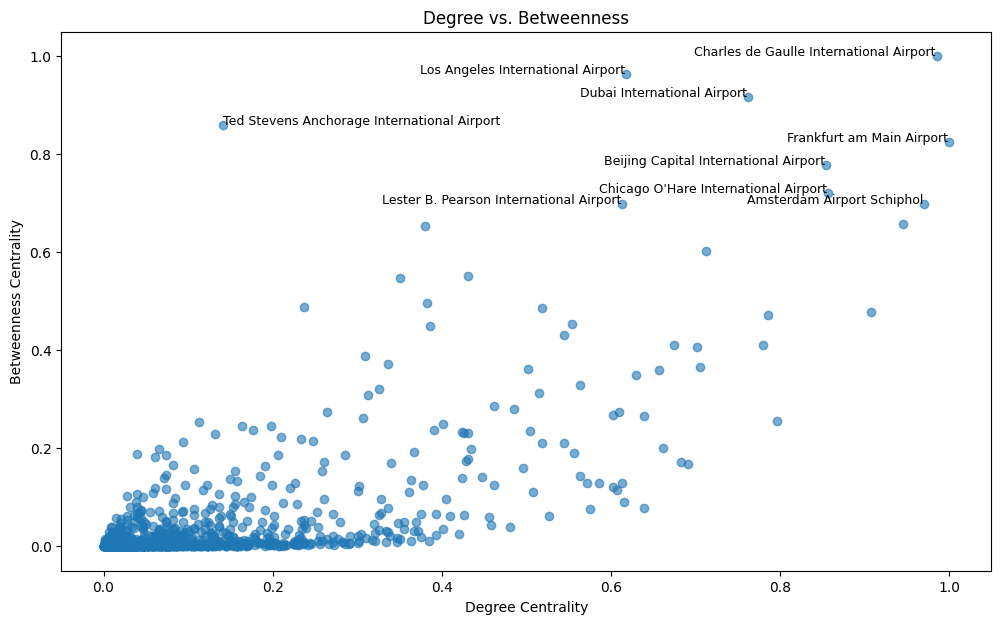
\includegraphics[width=1\textwidth]{images/degree_vs_betw.png}
    \caption{\centering Vzťah medzi Degree centrality a Betweenness centrality pre uzly globálnej leteckej siete.}
    \label{fig:degree_vs_betweenness}
\end{figure}

Graf odhaľuje výraznú heterogenitu funkčných rolí letísk v globálnej leteckej sieti. Väčšina uzlov je koncentrovaná v ľavej dolnej časti 
grafu, čo naznačuje nízku konektivitu aj obmedzený tranzitný význam. Len malý počet letísk vystupuje ako systémovo dominantné uzly s vysokými 
hodnotami oboch metrík.

Výrazným outlierom je letisko \textbf{Ted Stevens Anchorage International Airport}, ktoré sa nachádza izolovane v ľavej hornej časti grafu. 
Napriek relatívne nízkej degree centralite dosahuje mimoriadne vysokú hodnotu \textit{Betweenness centrality}, čo potvrdzuje jeho úlohu strategického 
tranzitného mosta medzi Áziou a Severnou Amerikou. Anchorage tak predstavuje typ uzla, ktorého význam nevyplýva z množstva spojení, ale z kontroly nad 
kritickými najkratšími cestami v sieti. Je zahrnuté v Národnom pláne integrovaných letiskových systémov Federálnej leteckej správy USA, kde je zaradené
do kategórie primárnych komernčných letísk strednej veľkosti. Z hľadiska nákladnej dopravy sa radí medzi najvyťaženejšie letiská na svete \footnote{Zdroj: $https://en.wikipedia.org/wiki/Ted\_Stevens\_Anchorage\_International\_Airport$}.

Naopak, letiská ako \textbf{Charles de Gaulle}, \textbf{Frankfurt} a \textbf{Amsterdam Schiphol} sa nachádzajú v pravom hornom 
rohu grafu, kde kombinujú vysokú mieru konektivity aj vysoký tranzitný význam. Tieto uzly tvoria jadro globálnej leteckej siete a predstavujú 
systémovo najintegrovanejšie huby.

Zaujímavú skupinu tvoria aj letiská ako \textbf{Beijing Capital International Airport} a \textbf{Chicago O'Hare International Airport}, 
ktoré síce disponujú vysokou konektivitou, no v porovnaní s európskymi hubmi dosahujú nižšie hodnoty \textit{Betweenness centrality}. To naznačuje 
odlišný charakter ich sieťovej funkcie, orientovaný viac na regionálnu distribúciu než na globálny tranzit.

\section{Analýza kompozitných indexov}

\subsection{Globálne systémové huby}

Na základe kompozitného indexu \textit{Global Hub Score} sme identifikovali uzly s najvyššou mierou systémovej dôležitosti. Tieto letiská predstavujú 
kritickú infraštruktúru, pričom ich dominancia je stabilná naprieč viacerými metrikami.

\begin{table}[h!]
\centering
\small
\begin{tabular}{cllc}
\hline
\textbf{Poradie} & \textbf{Názov letiska} & \textbf{Lokalita} \\ \hline
1. & Charles de Gaulle International Airport & Paríž, FR \\
2. & Frankfurt am Main Airport & Frankfurt, DE \\
3. & Amsterdam Airport Schiphol & Amsterdam, NL \\
4. & Atatürk International Airport & Istanbul, TR \\
5. & Dubai International Airport & Dubaj, AE \\
6. & London Heathrow Airport & Londýn, GB \\
7. & Beijing Capital International Airport & Peking, CN \\
8. & Chicago O'Hare International Airport & Chicago, US \\
9. & Munich Airport & Mníchov, DE \\
10. & Los Angeles International Airport & Los Angeles, US \\ \hline
\end{tabular}
\caption{\centering Top 10 letísk podľa Global Hub Score (všestranná sieťová dominancia).}
\label{tab:top10_global_hubs}
\end{table}

V prvej desiatke dominuje európsky región (6 z 10 letísk). Významné je 
zastúpenie letiska v Dubaji, ktoré vďaka svojej strategickej polohe medzi Európou a Áziou maximalizuje tranzitný potenciál napriek menšiemu 
vnútroštátnemu trhu v porovnaní s americkými letiskami.


\subsection{Strategické premostenie}

Výsledky aplikácie \textit{Bridge Indexu} (Tabuľka \ref{tab:bridge_index}) odhaľujú konkrétne uzly, ktoré fungujú ako kritické úzke hrdlá siete.
Tento index zvýrazňuje uzly, ktoré pri nízkom počte spojení kontrolujú disproporčne veľké množstvo tranzitných trás. Tieto letiská predstavujú 
miesta, kde je sieť najviac zraniteľná.

\begin{table}[h!]
\centering
\small
\begin{tabular}{cll}
\hline
\textbf{Poradie} & \textbf{Názov letiska} & \textbf{Región} \\ \hline
1. & Ted Stevens Anchorage & Aljaška, USA \\
2. & Minaçu Airport & Brazília \\
3. & Thunder Bay Airport & Ontário, Kanada \\
4. & Bangoka International & DR Kongo \\
5. & Fort Albany Airport & Ontário, Kanada \\
6. & Norman Wells Airport & SZ Teritóriá, Kanada \\
7. & Kangerlussuaq Airport & Grónsko \\
8. & Moosonee Airport & Ontário, Kanada \\ 
9. & Redenção Airport & Brazília \\ 
10.& Gurupi Airport & Brazília \\ \hline
\end{tabular}
\caption{\centering Top letiská podľa Bridge Indexu (Kritické sieťové mosty).}
\label{tab:bridge_index}
\end{table}

Analýza \textit{Bridge Indexu} identifikovala dve fundamentálne odlišné skupiny uzlov. Prvou sú globálne tranzitné mosty ako \textbf{Anchorage} 
a \textbf{Kangerlussuaq}, ktoré slúžia ako nevyhnutné technické zastávky pre transkontinentálne lety. 

Druhú, početnejšiu skupinu, tvoria letiská v odľahlých oblastiach Kanady, Brazílie a Afriky (napr. \textbf{Fort Albany} alebo \textbf{Minaçu}). Tieto uzly 
reprezentujú kritické body, ktorých výpadok by viedol k úplnej izolácii priľahlých komunít. Ich vysoký 
index je daný tým, že sú jediným prístupovým bodom do rozsiahlych geografických oblastí, čo z nich robí strategické priority z hľadiska národnej 
infraštruktúry.


\subsection{Regionálne centrá a akumulátory (Regional Index)}

Analýza regionálnej akumulácie (Tabuľka \ref{tab:regional_index_results}) ukazuje dominanciu európskych uzlov.
Tieto letiská disponujú extrémnym počtom linkových  spojení, ktoré však nie sú nevyhnutné pre globálnu integritu transkontinentálnych trás.

\begin{table}[h!]
\centering
\small
\begin{tabular}{cll}
\hline
\textbf{Poradie} & \textbf{Názov letiska} & \textbf{Lokalita} \\ \hline
1. & London Stansted Airport & Londýn, GB \\
2. & Munich Airport & Mníchov, DE \\
3. & Düsseldorf Airport & Düsseldorf, DE \\
4. & London Gatwick Airport & Londýn, GB \\
5. & Barcelona International Airport & Barcelona, ES \\
6. & Vienna International Airport & Viedeň, AT \\
7. & Manchester Airport & Manchester, GB \\
8. & Brussels Airport & Brusel, BE \\
9. & Dublin Airport & Dublin, IE \\
10. & Palma De Mallorca Airport & Palma de Mallorca, ES \\ \hline
\end{tabular}
\caption{\centering Top 10 letísk podľa Regional Indexu.}
\label{tab:regional_index_results}
\end{table}

V tejto kategórii dominuje európsky kontinent, ktorý v prvej stovke najvýznamnejších regionálnych centier zastupuje až 56 \% uzlov. Vysoké hodnoty 
letísk ako \textbf{London Stansted Airport} alebo \textbf{London Gatwick Airport} sú výsledkom stratégie nízkonákladových dopravcov, ktorí budujú 
husté siete typu bod-bod (point-to-point). 

Z hľadiska sieťovej topológie tieto uzly fungujú ako „akumulátory“ – miesta, kde sa doprava sústreďuje, ale nepokračuje ďalej pri letoch medzi 
kontinentálnymi blokmi. Príkladom sú letiská \textbf{Barcelona International Airport} a \textbf{Palma De Mallorca Airport}, ktoré vykazujú vysokú 
mieru konektivity naviazanú na cestovný ruch. Hoci sú tieto letiská kľúčové pre ekonomickú stabilitu a mobilitu v rámci Európy, ich globálny tranzitný 
dosah je v porovnaní s uzlami typu Bridge výrazne nižší.


\subsection{Vnútroštátni giganti}

Index vnútroštátnej dominancie izoluje letiská, ktoré disponujú masívnou priamou konektivitou, no ich prepojenie na globálne „elitné“ 
jadro siete je relatívne slabšie. Tento ukazovateľ identifikuje uzly, ktoré profitujú z obrovských vnútroštátnych trhov, pričom ich topologický vplyv
 na medzinárodnú prestíž systému je v porovnaní s ich veľkosťou sekundárny.

\begin{table}[h!]
\centering
\small
\begin{tabular}{cll}
\hline
\textbf{Poradie} & \textbf{Názov letiska} & \textbf{Lokalita} \\ \hline
1. & Hartsfield Jackson Atlanta International Airport & Atlanta, US \\
2. & Denver International Airport & Denver, US \\
3. & Dallas Fort Worth International Airport & Dallas/Fort Worth, US \\
4. & Guangzhou Baiyun International Airport & Guangzhou, CN \\
5. & Beijing Capital International Airport & Peking, CN \\
6. & Domodedovo International Airport & Moskva, RU \\
7. & Chicago O'Hare International Airport & Chicago, US \\
8. & George Bush Intercontinental Houston Airport & Houston, US \\
9. & Kunming Changshui International Airport & Kunming, CN \\
10. & Chengdu Shuangliu International Airport & Chengdu, CN \\ \hline
\end{tabular}
\caption{\centering Top 10 letísk podľa Local Giant Indexu.}
\label{tab:local_giant_index}
\end{table}

Výsledky tohto indexu odhaľujú zásadný rozdiel medzi objemom konektivity a globálnou prestížou. V rebríčku dominujú výhradne letiská z krajín 
s rozsiahlou geografickou rozlohou a silným domácim trhom, konkrétne \textbf{Čína (33 letísk v Top 100)} a \textbf{Spojené štáty (24 letísk v Top 100)}. 

Letiská ako \textbf{Hartsfield Jackson Atlanta International Airport} alebo \textbf{Beijing Capital International Airport} obsluhujú extrémne 
množstvo spojení, čo ich radí na vrchol svetových rebríčkov v počte letov. Avšak ich nižšia hodnota v rámci \textit{Eigenvector centrality} 
(prestíže) v porovnaní s európskymi hubmi naznačuje, že veľká časť ich siete je uzavretá vnútri národných systémov. Tieto uzly sú kľúčové pre 
ekonomickú stabilitu svojich krajín.


\subsection{Exkluzívne satelitné uzly}

Index sieťovej prestíže identifikuje takzvané „elitné satelity“. Ide o letiská, ktoré disponujú veľmi nízkym počtom priamych spojení, avšak tieto 
spojenia smerujú výhradne do najvýznamnejších globálnych hubov. Vysoká hodnota tohto indexu naznačuje, že uzol je napriek svojej malej fyzickej 
veľkosti priamou bránou do jadra globálneho systému.

\begin{table}[H]
\centering
\small
\begin{tabular}{cll}
\hline
\textbf{Poradie} & \textbf{Názov letiska} & \textbf{Lokalita} \\ \hline
1. & Filippos Airport & Kozani, GR \\
2. & Bolzano Airport & Bolzano, IT \\
3. & Salamanca Airport & Salamanca, ES \\
4. & Burgos Airport & Burgos, ES \\
5. & Leon Airport & León, ES \\
6. & Kastamonu Airport & Kastamonu, TR \\
7. & Nakhchivan Airport & Nachičevan, AZ \\
8. & Süleyman Demirel International Airport & Isparta, TR \\
9. & Mihail Kogălniceanu International Airport & Konstanca, RO \\
10. & Zafer Airport & Kütahya/Zafer, TR \\ \hline
\end{tabular}
\caption{\centering Top 10 letísk podľa Prestige Indexu.}
\label{tab:prestige_index}
\end{table}

V rebríčku Prestige Indexu absolútne dominuje \textbf{Európa (74 letísk v Top 100)}. Tento výsledok reflektuje špecifickú štruktúru európskeho letectva, 
kde aj veľmi malé regionálne letiská (napríklad v Grécku, Taliansku alebo Španielsku) disponujú priamymi linkami do kľúčových metropol ako Frankfurt, 
Paríž alebo Londýn.

Letiská ako \textbf{Bolzano Airport} alebo \textbf{Salamanca Airport} majú minimálnu \textit{Degree centralitu}, čo znamená, že obsluhujú len zlomok 
destinácií v porovnaní s veľkými hubmi. Avšak vďaka tomu, že ich jediní susedia v grafe sú uzly s najvyššou \textit{Eigenvector centralitou}, získavajú 
tieto satelity vysokú mieru topologickej prestíže. Z hľadiska sieťovej stratégie tieto body predstavujú efektívne kanály, ktoré umožňujú rýchly prístup 
z hlbokej periférie priamo do centra svetového diania bez potreby viacerých prestupov v rámci regionálnej siete.